

\subsection{Grafiken und Animationen}
Jede der Spielszenen hat drei Grafik-Assets: eine Intrografik für die Szenenlobby, einen Hintergrund für den Kampfbildschirm und eine Bossgegner-Grafik mit 2D-Animationen. Zudem kommt noch eine weitere Grafik für die Weltkarte hinzu. Diese Letztere, Intro und Hintergrund besitzen das JPG-Bildformat. Die Bossgegner-Grafik dagegen ist ein MP4-Video.
\\Für das JPG-Format entschieden wir uns hauptsächlich auf Grund der im Vergleich zu PNG geringeren Dateigröße. Da es sich bei allen Grafiken, um rein statische Bilder handelt, erschien der Komprimierungsverlust von jpg vernachlässigbar. Zudem wurde für die Bilder keine Hintergrund-Transparenz benötigt.
Alle Grafiken wurden in einer Auflösung von 3840x2160 (Ultra-HD) gezeichnet und dann entweder so verwendet oder auf 1920x1080 (Full-HD) herabskaliert.

\begin{figure}[H]
    \centering
     \label{fig:mine_exterior_concept}
     \caption{Vom Concept Art zur finalen Grafik}
     \subfloat[][]{\fbox{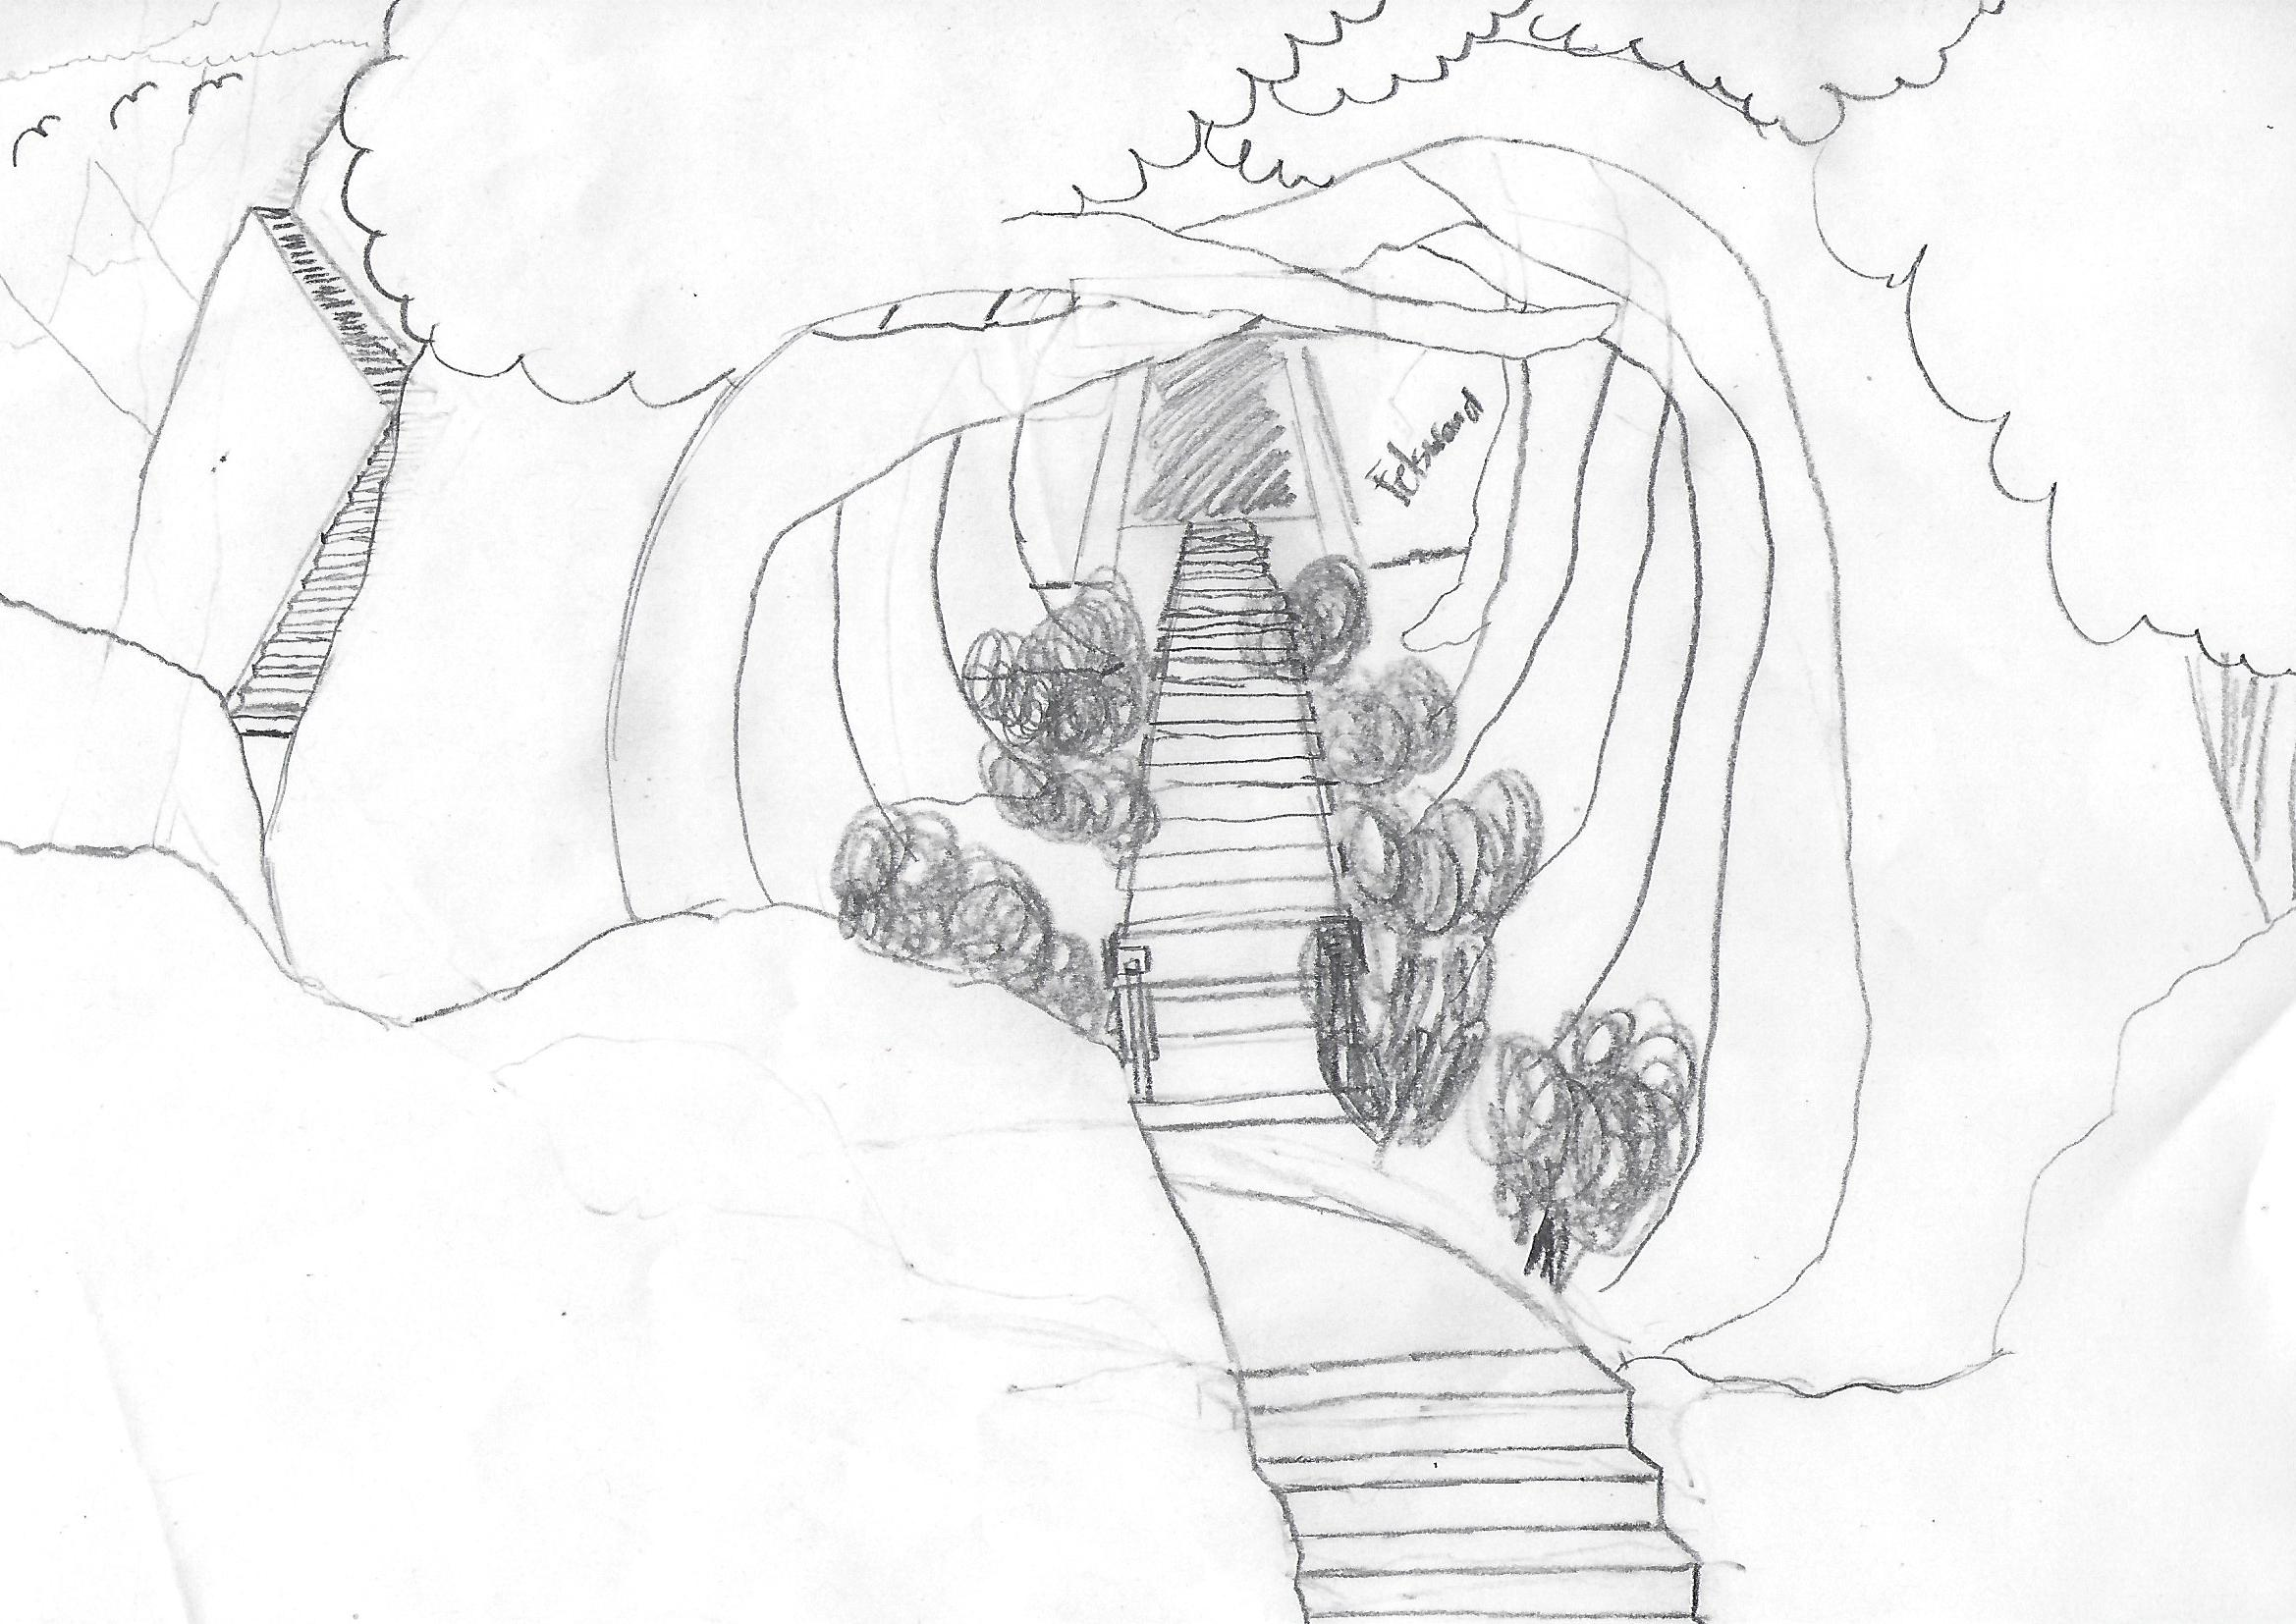
\includegraphics[width=0.5\linewidth]{mine_exterior_concept}}}
     \subfloat[][]{\fbox{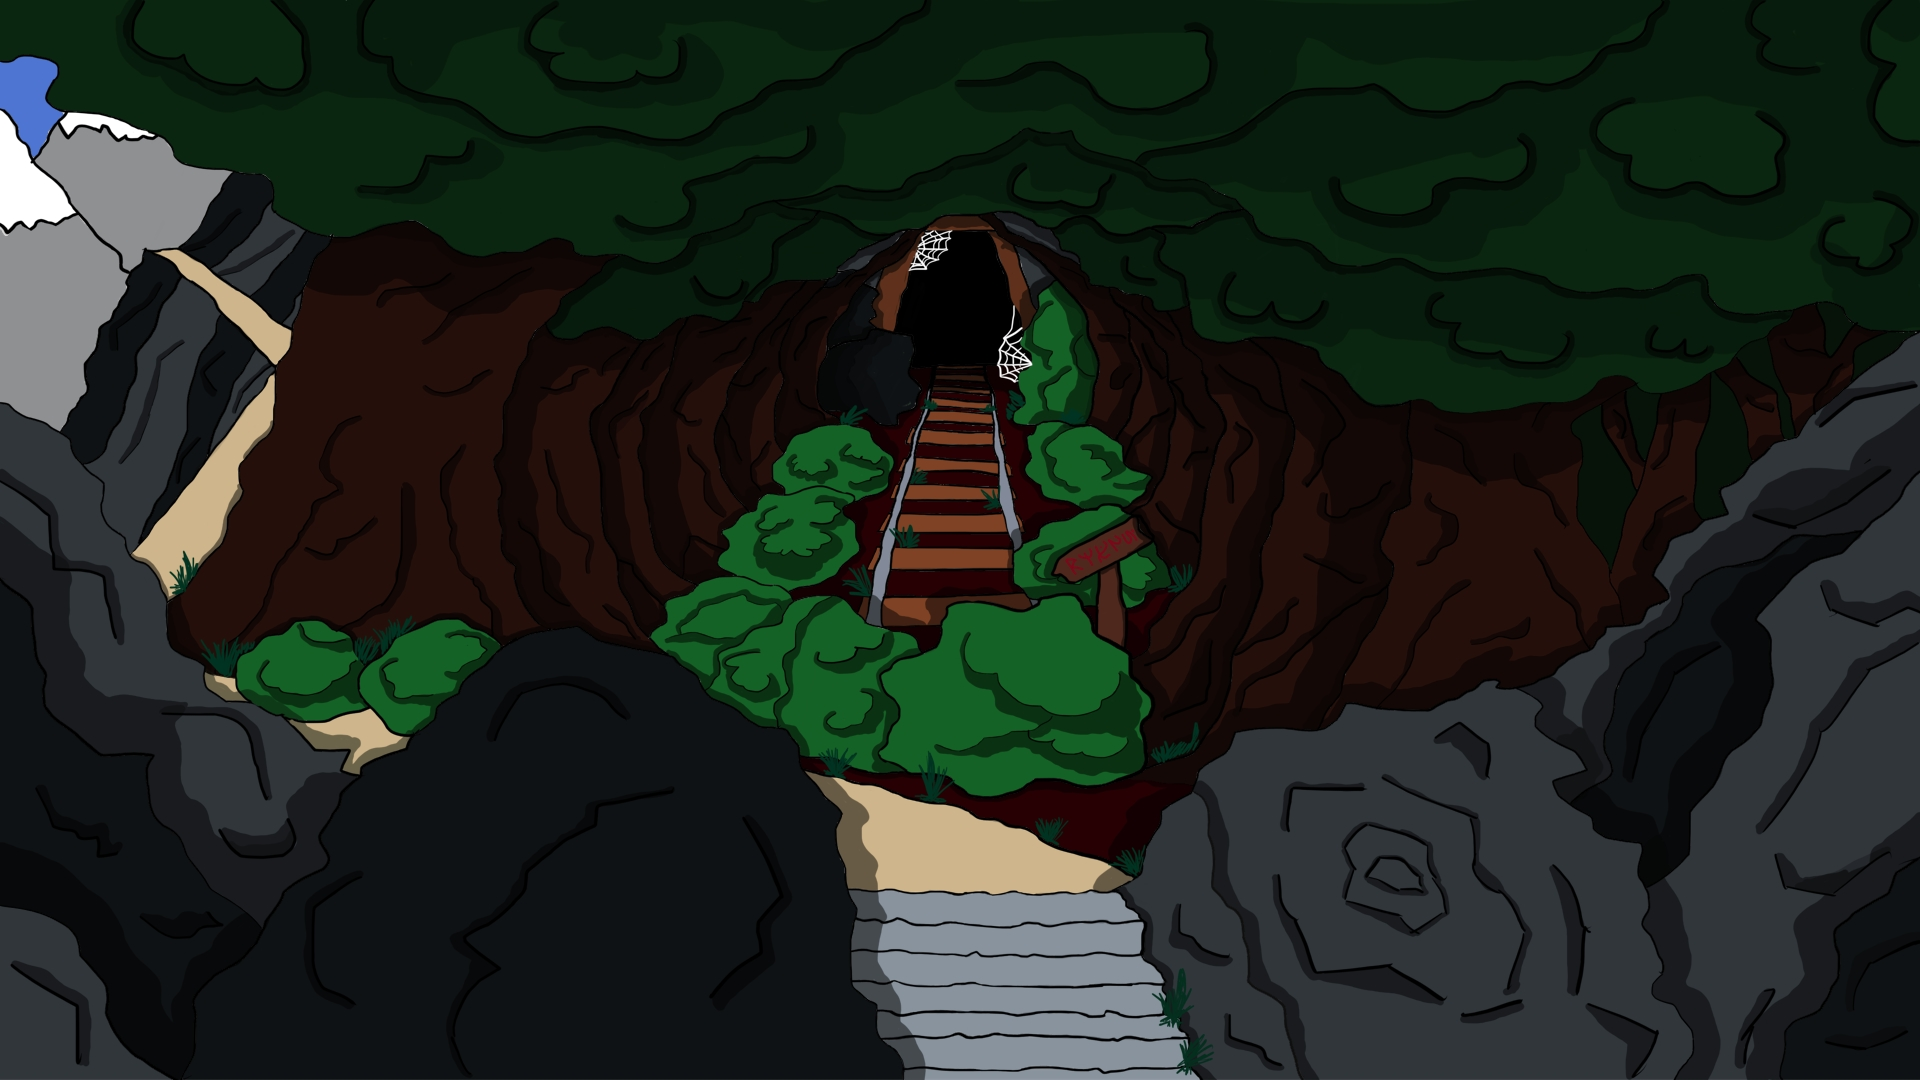
\includegraphics[width=0.5\linewidth]{mine_exterior_final}}}
  \end{figure}

Für die Erstellung der Grafik-Assets und Animationen wurden das freie Zeichen- und 2D-Animationsprogramm \textit{Krita}\footnote{siehe https://krita.org/en/} und ein Grafiktablet verwendet (in der folgenden Abbildung beispielhaft das Standard-UI von Krita).   

\begin{figure}[H]
    \centering
    \caption{Krita Standard-UI}
    \label{fig:krita_ui_example}
    \fbox{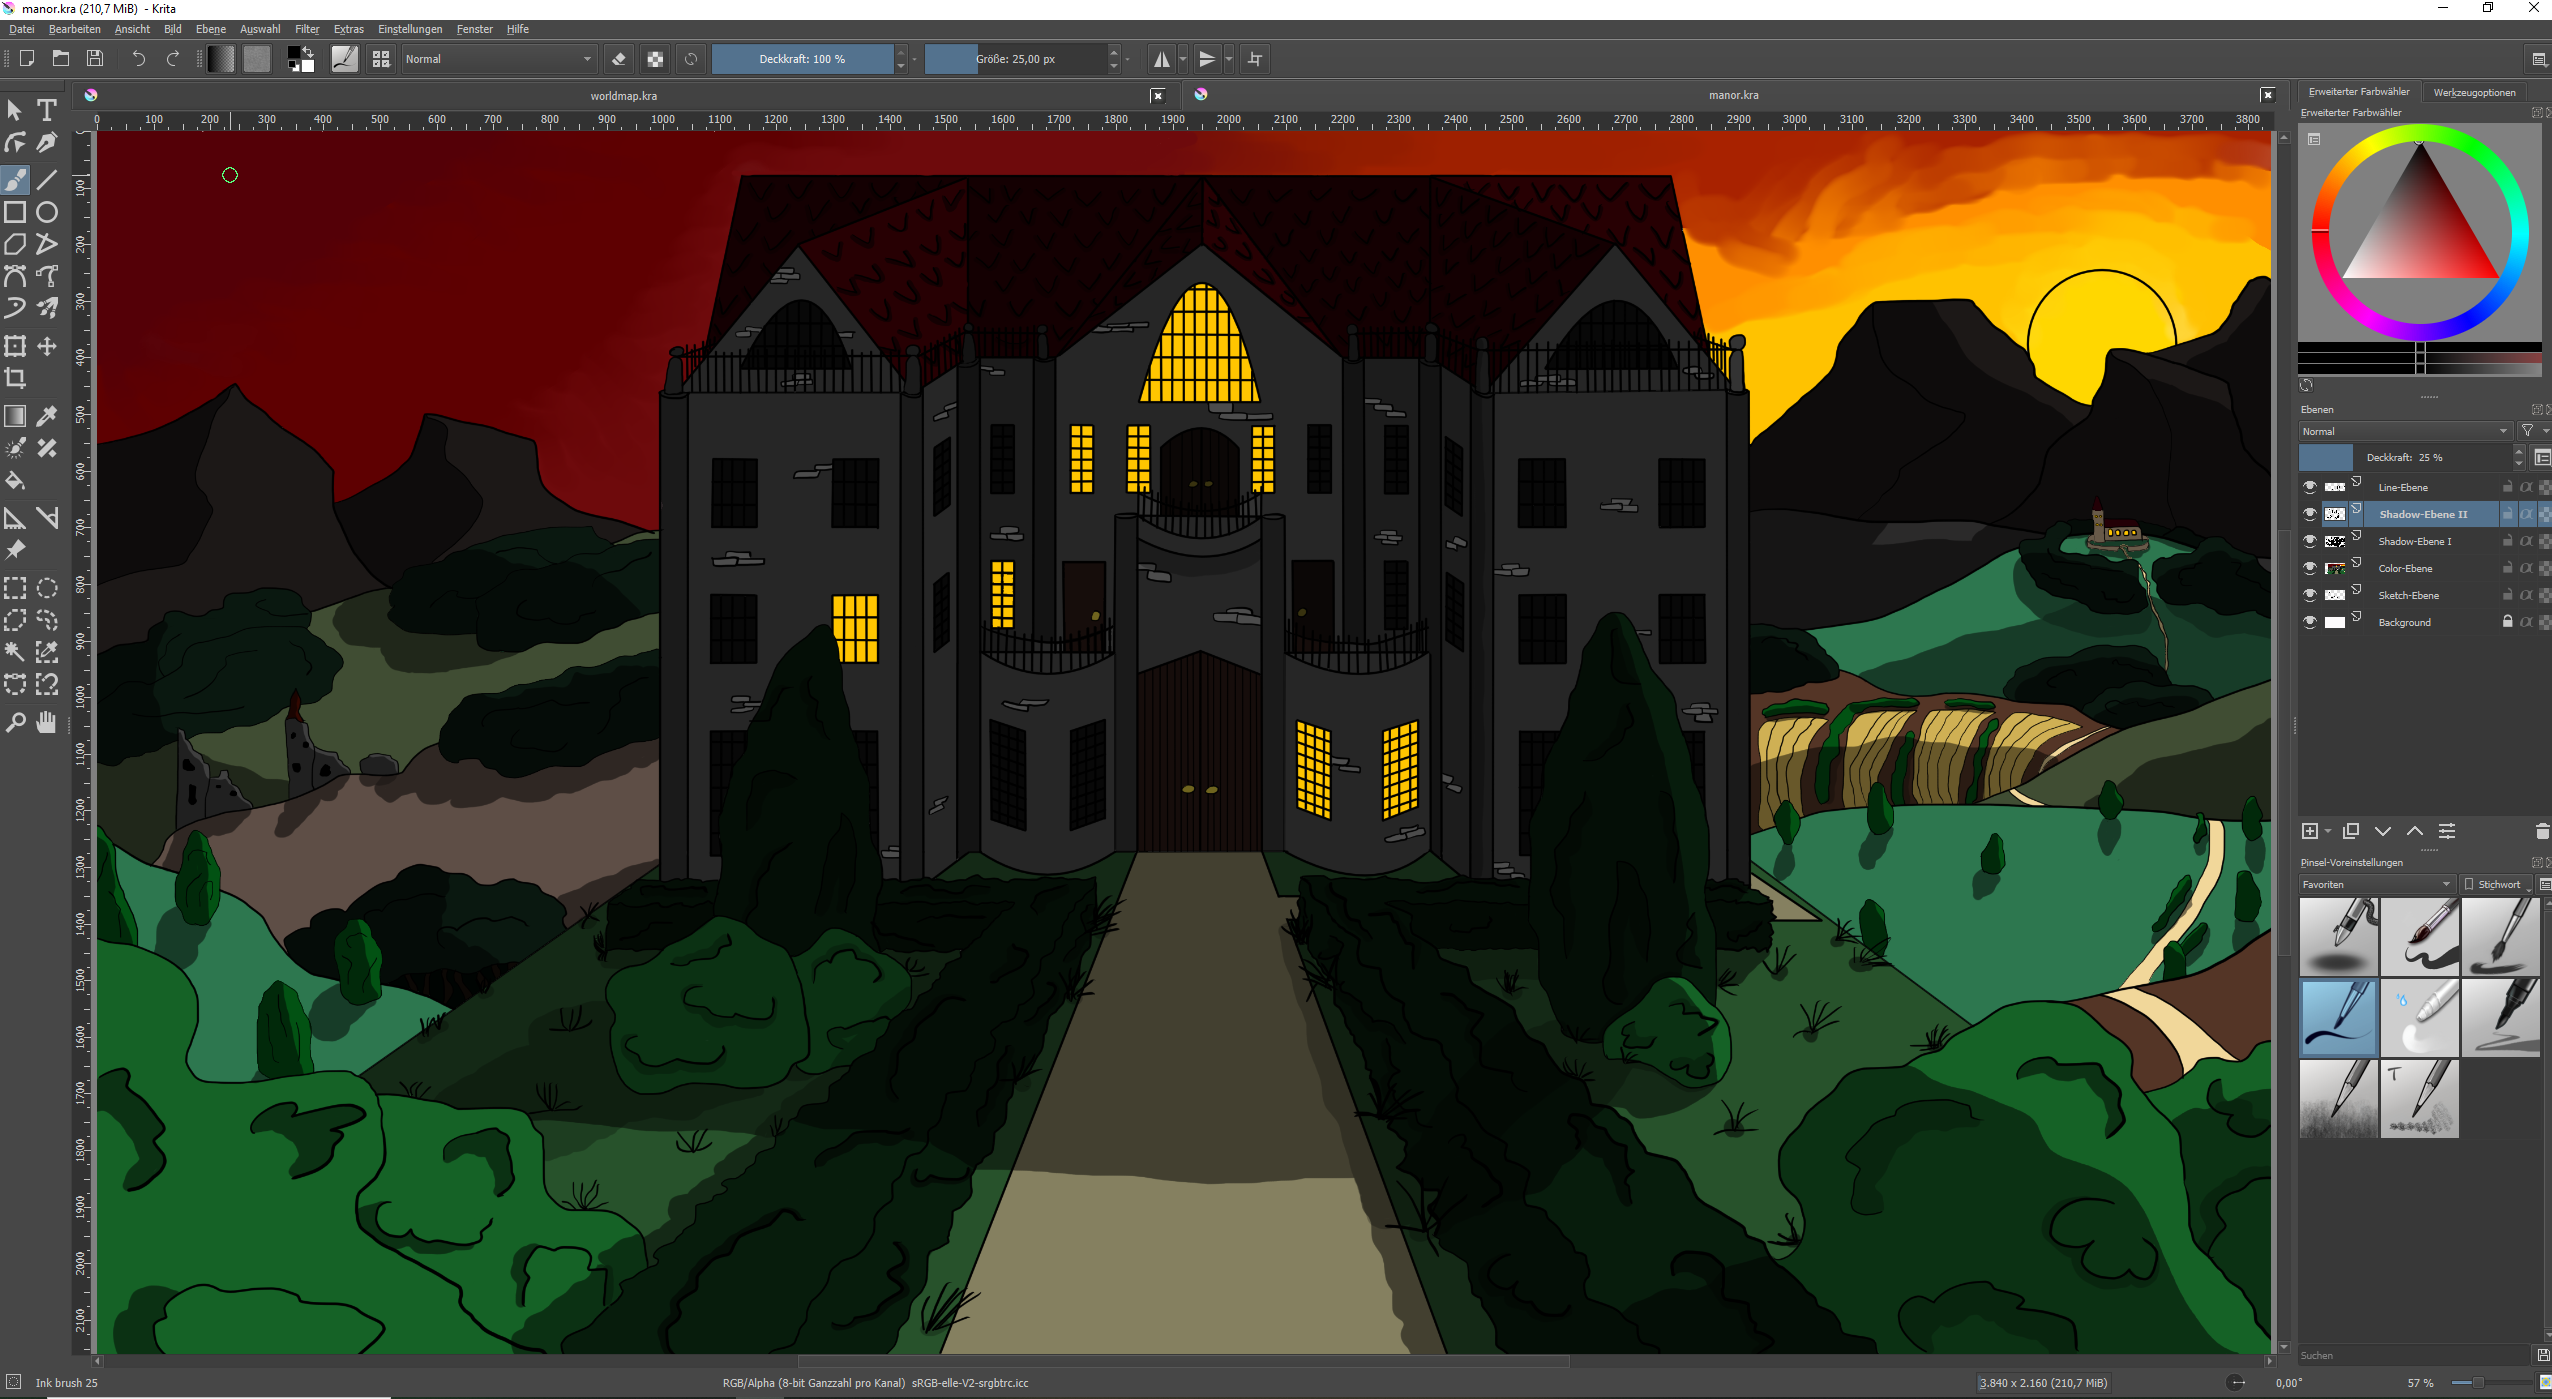
\includegraphics[width=1\textwidth]{krita_ui_example}}
\end{figure}

Die Grafiken wurden hierbei mithilfe der softwareeigenen Ebenenhierarchie systematisch wie folgt aufgebaut: 

Eine Konzeptzeichnung bildet die unterste Ebene mit einer vergleichsweise geringen Deckkraft (\enquote{Sketch-Ebene}). Darüber folgt die \enquote{Linien-Ebene}, auf der auf Basis der Skizze eine vollständige Strichzeichnung mit maximaler Deckkraft angefertigt wird. Diese bildet die oberste Ebene und alle folgenden Ebenen werden aufsteigend zwischen diesen beiden positioniert. Durch eine sorgfältige Linienführung auf dieser Ebene kann das Fülltool auf der nun folgenden \enquote{Farb-Ebene} effektiv genutzt werden. Den Abschluss bilden ein oder zwei \enquote{Schatten-Ebenen}, die mit einer Deckkraft von 50\% bzw. 25\% über der eigentlichen Kolorierung liegen. 

Im Falle der Bossgegner-Grafiken wird dieses Konzept noch um drei Gruppen ergänzt, welche jeweils alle Ebenen in sich zusammenfassen. Es gibt eine Gruppe für das Hintergrundbild, eine Gruppe für die nicht-aninimierten Teile des Bossgegners und eine Gruppe für die eigentlichen Animationen.
Zum Vergleich ist im Folgenden eine Abbildung dieses Aufbaus zu sehen (hier beispielhaft eine Grafik mit 2D-Animation):

\begin{figure}[H]
    \centering
    \caption{Ebenenkonzept für die Grafiken}
    \label{fig:krita_layer_example}
    \fbox{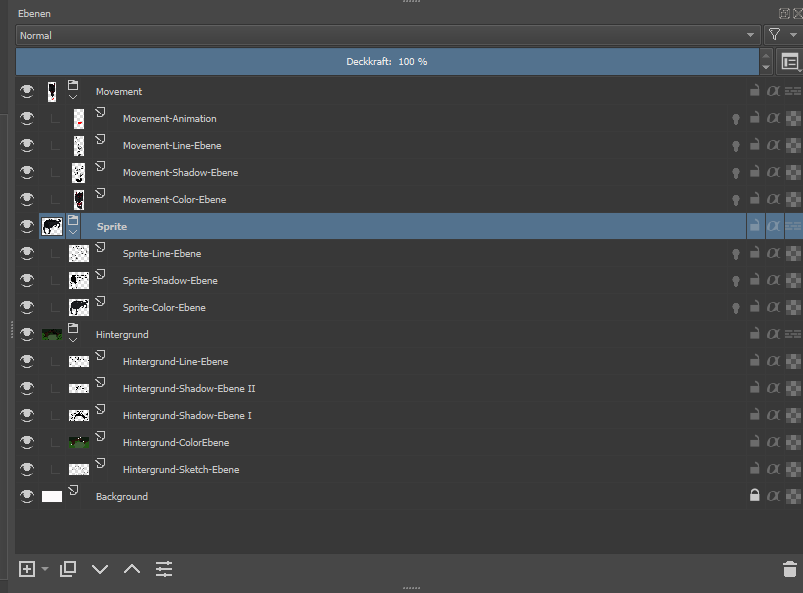
\includegraphics[width=0.7\textwidth]{krita_layer_example}}
\end{figure}

Dieses Konzept brachte eine erhebliche Flexibilität mit sich. Es war uns damit möglich effizient Änderungen an separaten Teilen der Grafiken durchzuführen, mit der Farbgebung zu experimentieren und nachträglich neue Details einzubringen. Zudem konnten Hintergrundbilder und Bossgrafiken als eine Datei erstellt werden und dann durch Ausblenden verschiedenener Ebenen individuell exportiert werden. Auch der Animationsprozess wurde durch diese Technik deutlich erleichtert. 

Für die Realisierung der 2D-Animationen bietet \textit{Krita} ein dediziertes User-Interface (siehe Abbildung unten). Die Ebenen können hier je nach Bedarf zusammen oder einzeln animiert werden. Dazu werden sie unabhängig voneinander in die Animationsframes kopiert und gegebenenfalls verändert. Im unten zu sehenden Beispiel werden die Ebenengruppen \enquote{Sprite} (nicht-animierter Teil der Bossgegner-Grafik) und \enquote{Movement} (eigentliche Animation) über 10 Frames hinweg durch sukzessive Erhöhung der Deckkraft eingeblendet, um den Effekt eines plötzliches Erscheinens aus Unsichtbarkeit zu erzielen. Danach wird in der \enquote{Movement}-Gruppe über 29 Frames eine Flügelbewegung realisiert. Die Animation wurde dann mit einer Bildwiederholrate von 10 Frames per Second gerendert und als MP4-Video in Ultra-HD und Full-HD exportiert. 

\begin{figure}[H]
    \centering
    \caption{Krita Animation UI}
    \label{fig:krita_animation_example}
    \fbox{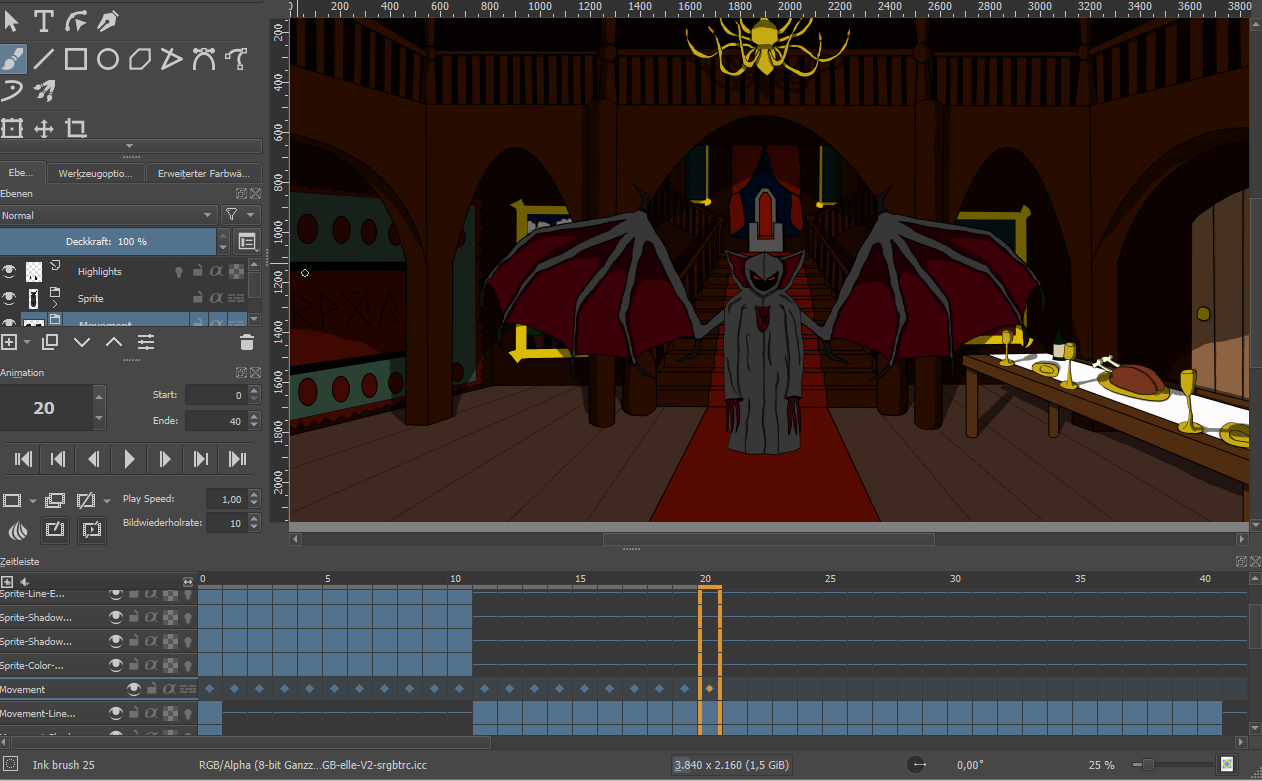
\includegraphics[width=1\textwidth]{krita_animation_example}}
\end{figure}

Die Separierung der Grafiken in animierte und nicht-animierte Teile, stellte bei der eigentlichen Animation eine erhebliche Arbeitserleichterung dar. Viele Bewegungsabläufe konnten durch Verschieben vorher definierter Abschnitte erreicht werden und mussten nicht pro Frame neu gezeichnet werden (teilweise wurde dies aber trotzdem nötig). Trotz dieser Erleichterung ergab sich aber immer noch ein erheblicher Arbeitsaufwand selbst für nur wenige Frames. Daher entschieden wir es bei vergleichsweise rudimentären Animationen zu belassen. Eine Realisierung in 30 Frames per Second beispielsweise wäre für das Projekt unverhältnismäßig zeitaufwendig gewesen.

Für die Ausgestaltung des Gamelogs und verschiedener Ambienttexte und die Darstellung der Klassen wurden vorgefertigte Emojii-Symbole von der Website \textit{emojiiterra}/footnote{siehe https://emojiterra.com} verwendet.

\pagebreak
\subsection{Frontend-Design}
Das im Rahmen dieses Projekts entstandene Spiel ist von klassischen Text-Adventures und Rollenspielen der Achtziger- und Neunzigerjahre inspiriert. Um den speziellen Look dieser Spiele zu treffen, entschieden wir uns, handgezeichnete Grafiken und eigene 2D-Animationen zu verwenden. Das Frontend-Design des Browserspiels sollte ebenfalls eine Hommage an diese Ära sein und dabei helfen den Charme dieser Ära einzufangen. 

Daher wählten wir das CSS-Framework \textit{RPGUI} von Ronen Ness\footnote{siehe https://github.com/RonenNess/RPGUI, veröffentlicht 2016 unter der zlib-Lizenz} als Basis der Gestaltung der Browserspiel-Oberfläche aus. Dieses Framework liefert eine große Anzahl vorgefertigter Klassen für verschiedenste HTML-Elemente im \enquote{Old-School-Look} klassischer 8-Bit und 16-Bit-RPG's. Neben dem eigentlichen CSS-Stylesheet werden zudem viele JavaScript-Funktionen bereitsgestellt, die z.B. die Benutzung von dynamischen Elementen wie einer Lebenspunkte-Anzeige ermöglichen.

\begin{figure}[H]
    \centering
    \caption{Frontend-Design Beispiel: Szenenlobby}
    \label{fig:frontend_rpgui_example}
    \fbox{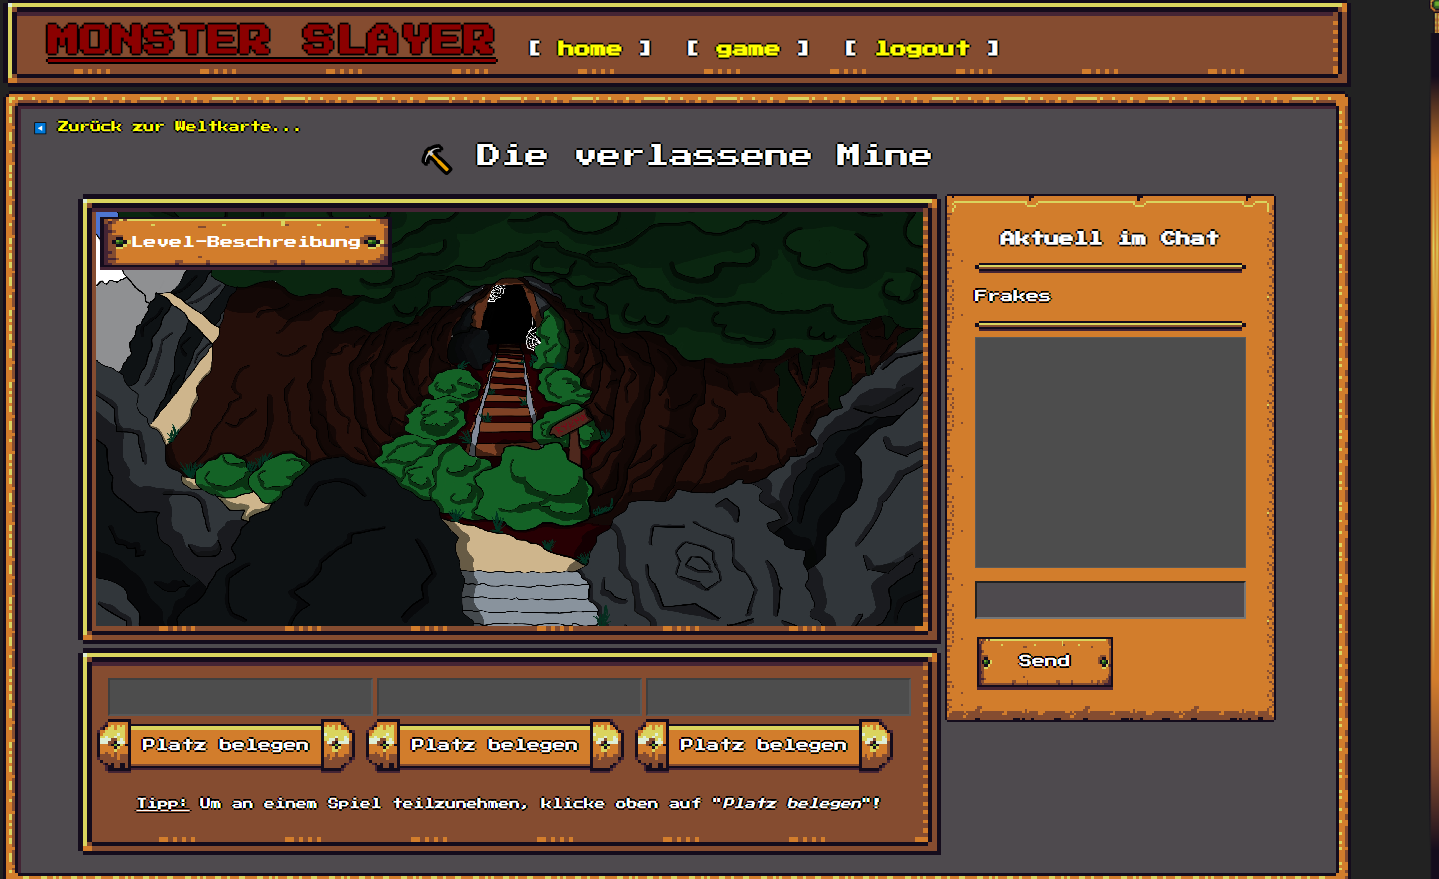
\includegraphics[width=0.7\textwidth]{frontend_rpgui_example}}
\end{figure}

Für die Implementation in das Frontend wurde zunächst dem übergeordnetem div-container in der \textit{base.html} die Klasse \textit{rpgui-content} zugeordnet. Dort sind grundlegende CSS-Stylings enthalten, die z.B. Schriftart, Schattierung, Hintergrundfarbe und Ausrichtung der Hintergrundbilder für die einzelnen Elemente definieren. Diese werden an weitere Elemente mit der Klasse \textit{rpgui-content-*} vererbt. Mithilfe der Template-Vererbung von Django via \textbf{extends} konnte so ein Großteil der Frontend-Gestaltung zentral in der \textit{base.html} vorgenommen werden.

Trotzdem war es in vielen Fällen notwendig Anpassungen an HTML-Elementen direkt in den Template-Dateien durchzuführen. Insbesondere für die Platzierung der Elemente auf der Webseite und die korrekte Skalierung für verschiedene Bildschirmgrößen wurde stark auf Inline-CSS zurückgegriffen. Dies sieht im Code dann wie folgt aus (Beispiel aus \textit{game\_endscreen.html}):

\begin{lstlisting}[language=html]
<div class="rpgui-container framed-golden" 
     style=" width: 50%;
             font-size: 1.4vw; 
             align-items: center;
             text-align: center;
             justify-content: center;
             margin-left: 25%; 
             margin-right:25%">
\end{lstlisting}

Hier wurde die von \textit{rpg-content} festgelegte font-size mit einem Viewport-Wert überschrieben, um eine bessere Skalierung zu ermöglichen. Zudem wurden im style-Element verschiedene Einstellung für das Seitenlayout vorgenommen. Dies wurde in ähnlicher Weise an vielen Stellen im Code so gemacht.

Wie oben erwähnt, wurden die meisten individuellen Einstellungen dafür verwendet, die Elemente skalierbar zu machen. Eines unserer Ziele für das Projekt war es, das Frontend zumindest bis zu einem gewissen Grad responsiv zu gestalten und so eine geräteübergreifende Nutzbarkeit des Spiels zu erreichen. So sollte beispielsweise innerhalb des Kampfbildschirms kein Scrollen notwendig sein. Es sollte sichergestellt werden, dass wichtige Steuerelemente, wie z.B. die Aktions-Buttons und der Gamelog, zu jedem Zeitpunkt vollständig sichtbar sind. Ein Scrollen und Suchen nach diesen Elementen erschien uns in Anbetracht der \enquote{Action-Szene}, in der sich die Spieler an diesem Punkt befinden, als der Immersion sehr abträglich. Daher wurde das overflow-Attribut für die gesamte \textit{game.html} und deren Tochter-Templates \textit{game\_content.html und game\_endscreen.html} deaktiviert und das Layout responsiv gestaltet. 

Hierfür war es zum Teil auch notwendig bestehende CSS-Klassen aus dem Framework anzupassen. Ein Nachteil des RPGUI-Frameworks ist die häufige Angabe von fixen Pixel-Maßen, die ein responsives Layout behindern. Im folgenden Code-Beispiel wird exemplarisch die angepasste RPGUI-Klasse \textit{rpgui-container.framed-scalable} gezeigt, welche aus der Originalklasse \textit{rpgui-container.framed} erstellt wurde:

\pagebreak
\begin{lstlisting}
    /* Skalierbare Elemente für game.html */
        .rpgui-container.framed-scalable {
    /* border */
        border-style: solid;
        border-image-source: url("img/border-image.png");
        border-image-repeat: repeat;
        border-image-slice: 6 6 6 6;
        border-image-width: 0.5vw;
        border-width: 0.4vw;
        padding-top: 0.8vh;
        padding-bottom: 0.8vh;
        padding-left: 0.8vh;
        padding-right: 0.8vh;
    /* internal border */
        box-sizing: border-box;
        -moz-box-sizing: border-box;
        -webkit-box-sizing: border-box;
    /* background */
        background: url("img/background-image.png") repeat repeat;
        background-clip: padding-box;
        background-origin: padding-box;
        background-position: center; }
\end{lstlisting}

Das Ziel der Skalierbarkeit haben wir grundsätzlich erreicht, es gibt allerdings gewisse Grenzen. Das UI wird auf Bildschirmen mit Tabletmaßen noch annehmbar skaliert - die für das Spielen nötigen Elemente sind bedienbar. Für das Spielen über ein Smartphone ist das Spiel allerdings nicht geeignet, da hier Elemente und Layout zu stark verschoben werden. Einer der Gründe hierfür ist die Verwendung von Viewport-Maßen (vh = viewport-height, vw = viewport-width; vgl. obiges Code-Beispiel) in unserem Frontend-Code. Diese Maße orientieren sich in ihrer Skalierung am Viewport des jeweiligen Gerätes (Viewport = Sichtfenster/Sichtöffnung/Display) und sorgen für eine theoretisch sehr effektive geräteübergreifende Anpassung. Die Angabe von fest vorgegebenen Viewport-Maßen im style-Element führt allerdings zu einer teilweise zu starken Verkleinerung bzw. Vergrößerung. Es müssten hier eigentlich individuelle Grenzen für jede Gerätegruppe gesetzt werden, was über sogenannte \enquote{Media Queries} erreicht werden kann. Uns ist diese Technologie bekannt, abr wir entschieden es trotzdem aus Aufwandsgründen bei der eher rudimentären geräteübergreifenden Skalierung zu belassen. Unser Hauptfokus lag während der Entwicklung eindeutig auf Notebook- und Desktop-Rechner Bildschirmgrößen und auf diesen verhält sich das UI korrekt responsiv.

In seltenen Fällen wurden von uns auch vollständig neue CSS-Klassen erstellt. Für den Spieltitel links oben in der Navigationsleiste wurde z.B. eine eigene Klasse \textit{game\_title} geschrieben. Durch die feste Vorgabe von grundlegenden Attributen wie font-size und color durch die \textit{rpgui-content} konnten wir den Titel nicht individuell formatieren. Auch Inline-CSS wird für diese Attribute überschrieben. Die Lösung war eine eigene Klasse zu erstellen und deren Attributsvorgaben mit \textbf{!important} zu kennzeichnen, was dazu führt, dass sie auch bei konkurrierenden Angaben eigentlich übergeordneter Klassen durchgesetzt werden.

\begin{lstlisting}
    .game_title{
        font-size: xx-large !important;
        color: #8B0000 !important;
        text-decoration: underline !important;
        /*border-style: solid !important;
        border-color: #8B0000 !important;
        border-radius: 25px !important;
        border-width: 7px !important;*/
        padding-top: 4px !important;
        padding-bottom: 4px !important;
        padding-left: 11px !important;
        padding-right: 4px !important;
        white-space: nowrap; }
\end{lstlisting}




    